%
% 02_Pitch_Detektion.tex
%
% (c) 2023 Florian Baumgartner, OST Ostschweizer Fachhochschule
%
% !TEX root = ../../buch.tex
% !TEX encoding = UTF-8
%
\section{Pitch-Detektion
\label{autotune:section:pitchDetektion}}
\rhead{Pitch-Detektion}
Bei einer einstimmigen Aufnahme, beispielsweise der menschlichen Stimme oder eines Blasinstruments,
wird nicht nur ein einzelner Ton erzeugt, sondern eine Reihe von Tönen, die als Obertöne oder Harmonische bezeichnet werden.
Die Grundharmonische ist der erste und stärkste dieser Töne, während die höheren Harmonischen in der Regel schwächer sind und höhere Frequenzen haben.
Es gilt nun die grundharmonische Frequenz zu finden die als dominante Tonhöhe wahrgenommen wird.
Es gibt mehrere Möglichkeiten dies umzusetzen.
Im Rahmen dieser Arbeit werden zwei Methoden verglichen.
Einerseits die Short-Time Fourier-Transformation (STFT) in Abschnitt \ref{autotune:subsection:shortTimeFourierTransformation},
andererseits die etwas unbekanntere Cumulative Mean Normalized Difference Function (CMNDF) in Abschnitt \ref{autotune:subsection:cumultativeMeanNormalizedDifferenceFunction}.

Grundsätzlich gilt, je genauer die Tonhöhe bestimmt werden kann, desto besser kann die Tonhöhe anschliessend korrigiert werden.
Die spektrale Frequenzauflösung ist ein direktes Mass für die Genauigkeit der Tonhöhenbestimmung.
So ist es möglich den maximalen Fehler der Frequenzabweichung zu bestimmen, der bei der Pitch-Detektion entstehen kann.

\subsection{Short-Time Fourier-Transformation (STFT)
\label{autotune:subsection:shortTimeFourierTransformation}}
Die Short-Time Fourier-Transformation (STFT) ist eine Fourier-Transformation, die auf einem kleinen,
zeitlich begrenzten Ausschnitt eines Signals angewendet wird.
Da es sich um einen diskreten Vorgang handelt, wird die STFT beschrieben als
\begin{equation}
    \mathbf{STFT}_x(m, f)
    =
    \sum_{n=-\infty}^{\infty}x(n)\;w(n-m)\;e^{-j 2 \pi f n}.
\end{equation}
Dabei definiert $x(n)$ das Signal, $w(n)$ das Fenster und $m$ den Verschiebungsparameter.
Üblicherweise wird ein Fenster der Länge $N$ verwendet, wobei $N$ eine Zweierpotenz ist.
Je länger das Zeitfenster, desto höher ist die physikalische Frequenzauflösung. Jedoch reduziert sich die zeitliche Spektrumabtastung.
Dieser Trade-Off kann gut anhand des Beispiels \ref{autotune:beispiel:tradeOffSTFT} gezeigt werden.
\begin{beispiel} 
    \[
        f_s = 44100\;\text{Samples/s} \quad\quad l_w = 23\;\text{ms} \quad\quad L = f_s \cdot l_w = 1014.3 \approx 1024\;\text{Samples}
    \]
    \[
        \Delta f = \frac{f_s}{L}\approx 43.07\;\text{Hz}
    \]
    \label{autotune:beispiel:tradeOffSTFT}
\end{beispiel}
Es fällt auf, dass mit einer Fensterlänge von 23\;ms die Frequenzauflösung bei nur 43.07\;Hz liegt.
Da einzelne Töne jedoch nur wenige Hertz auseinander liegen, können diese nur ungenau voneinander unterschieden werden.
Schnelle Melodien verhindern das Verlängern der Fensterzeit, da sonst mehrere Töne in ein Segment fallen und nicht mehr identifiziert werden können.

Bei einer Fensterlänge von 23\;ms wird das Spektrum also ca. 43 mal pro Sekunde abgetastet.
Wie in Abbildung \ref{autotune:fig:pitchDetektionSTFT} zu sehen ist, können somit auch schnelle Tonhöhenänderung erkannt werden.
\begin{figure}
	\centering
	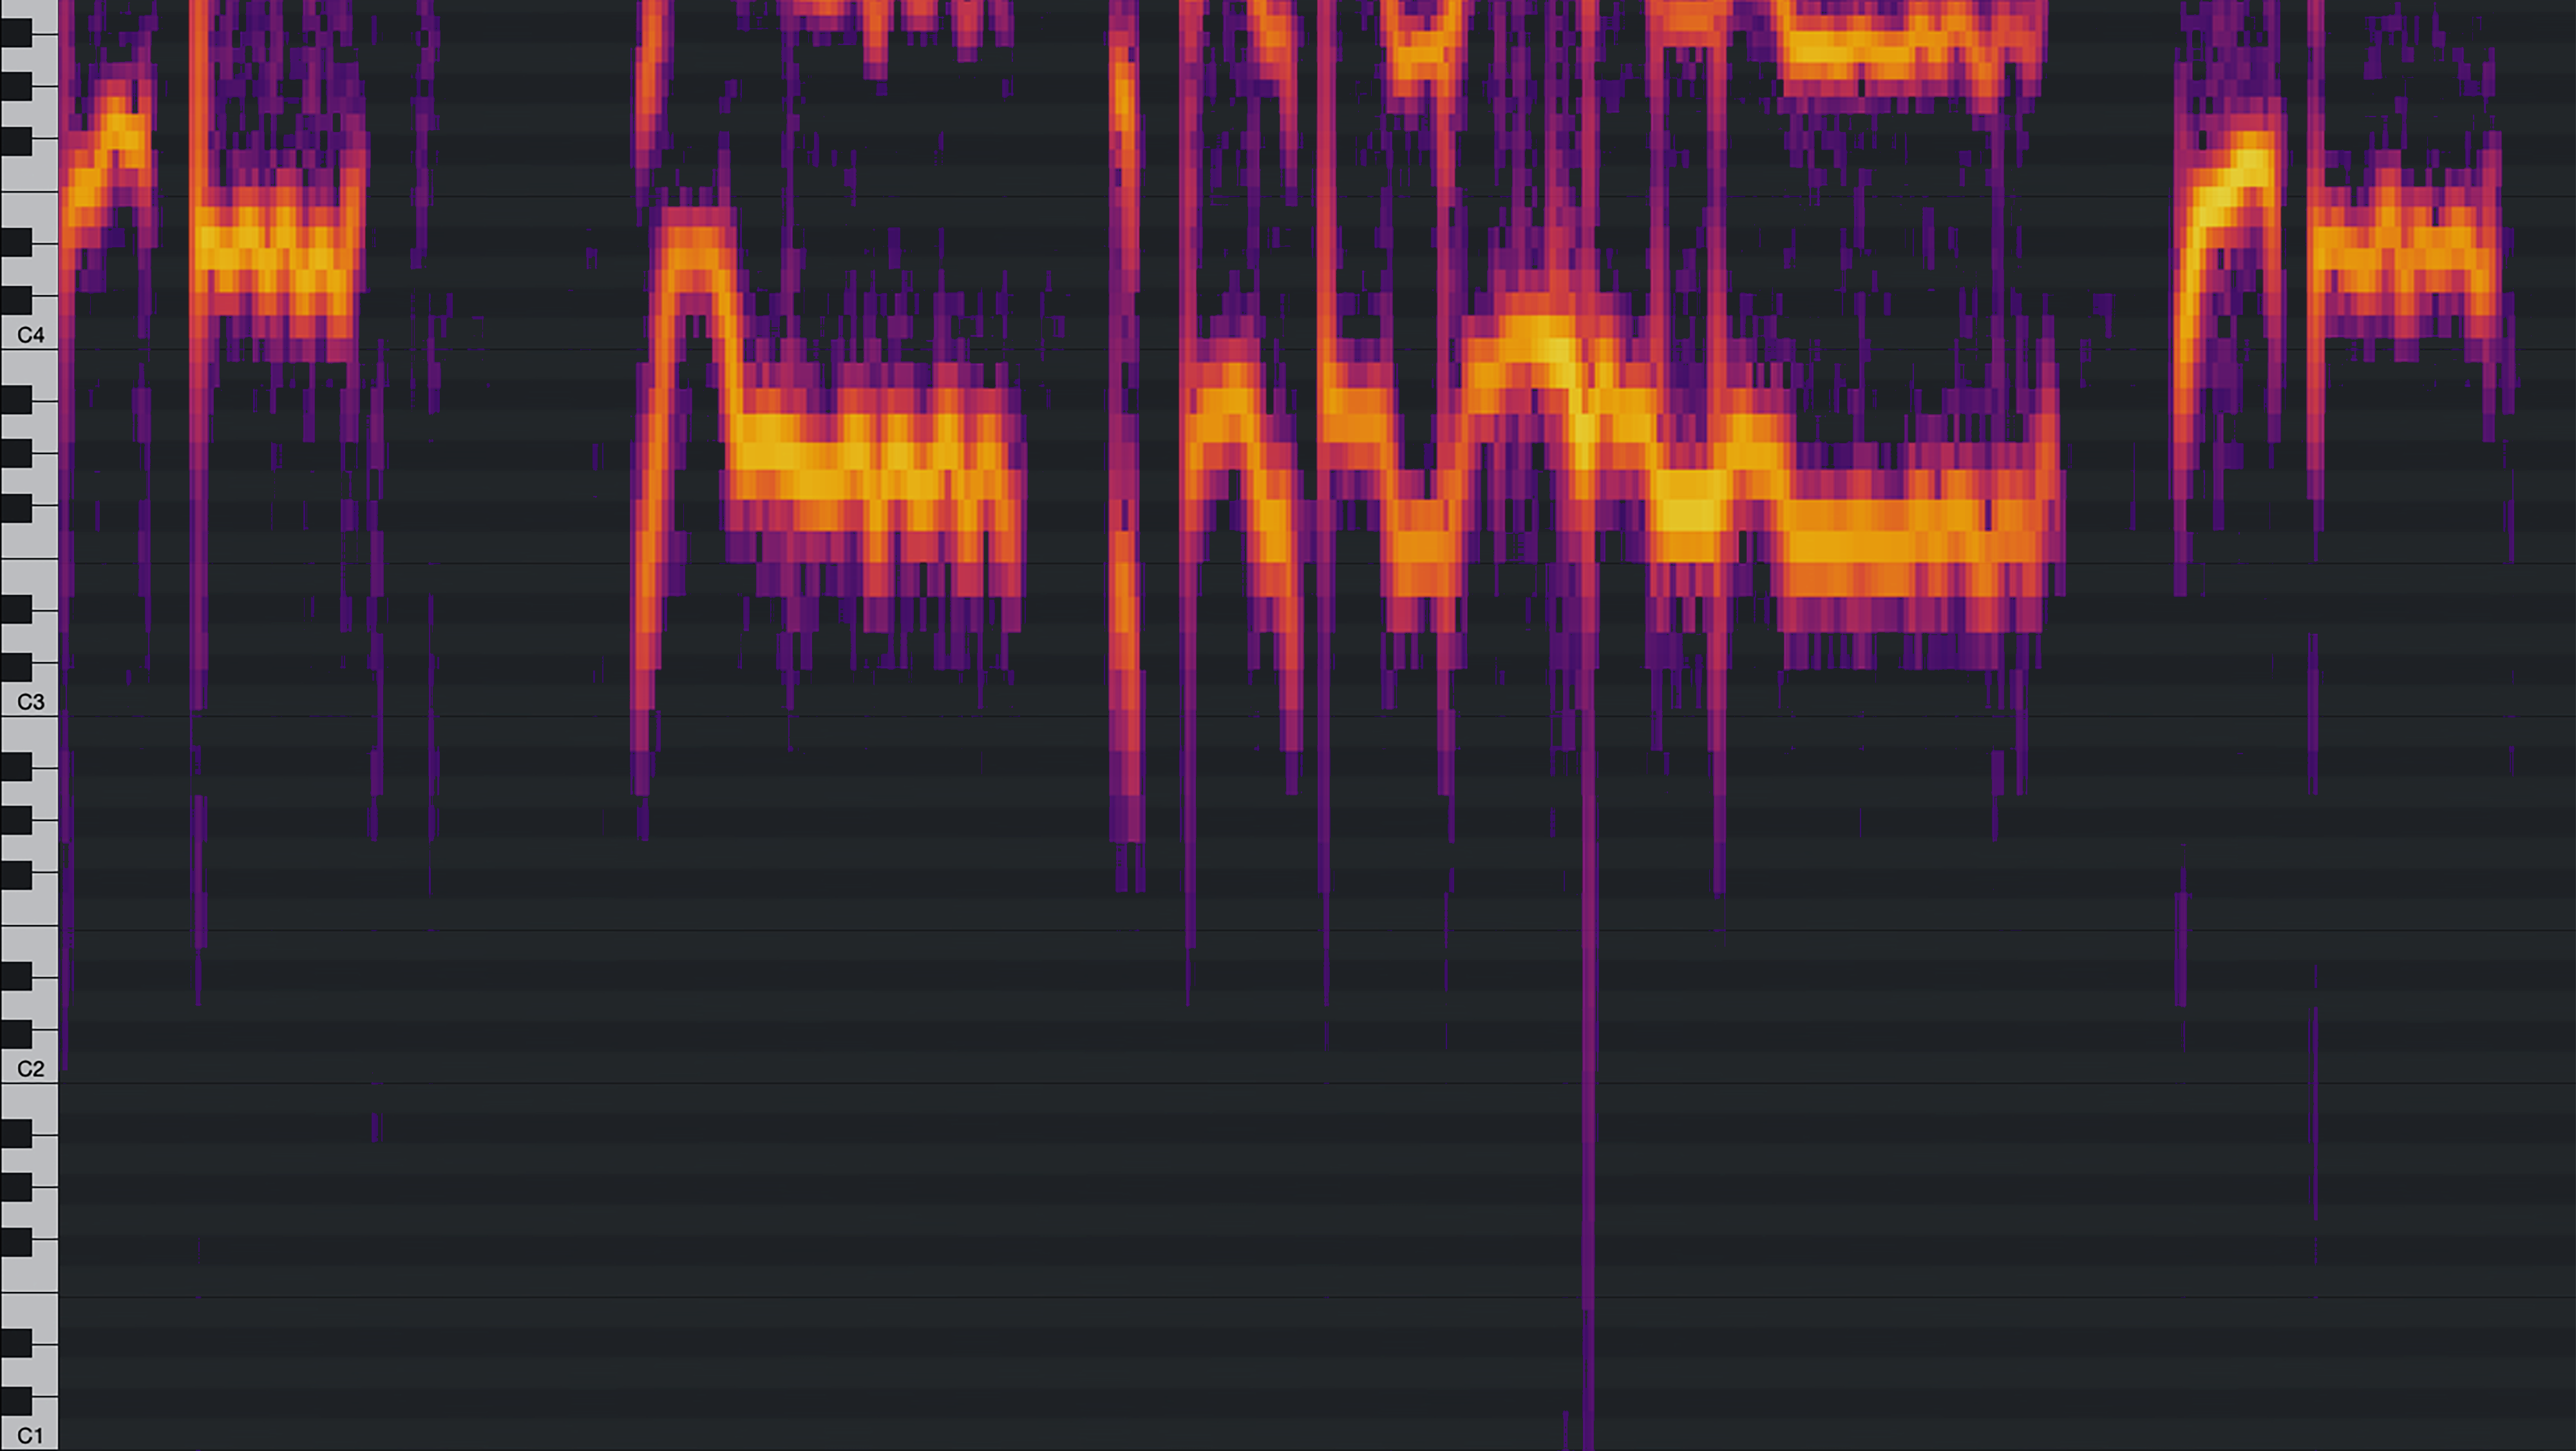
\includegraphics[width=\textwidth]{papers/autotune/images/Pianoscale_Example_Detuned_STFT.png}
	\caption{Pitch-Detektion mit STFT (Fensterlänge von 23\;ms).}
    \label{autotune:fig:pitchDetektionSTFT}
\end{figure}

Diese spektrale Darstellungsweise wird auch als Sonogramm bezeichnet.
Mehr dazu im Kapitel \ref{chapter:sonogramm}.

Das konkrete Bestimmen der Tonhöhe innerhalb eines Fensters kann auf verschiedene Arten umgesetzt werden.
Eine Möglichkeit zur Bestimmung der Grundharmonischen ist das Finden des Maximums im Spektrum (Peak-Detektor).
Mathematisch ausgedrückt als
\begin{equation}
    f_{\text{pitch}}
    =
    \arg\max_f \left| \; \mathbf{STFT}_x(m, f) \; \right|^2.
\end{equation}
Mit den konkreten Werten aus dem zuvor genannten Beispiel ergibt sich ein maximaler Frequenzabtastfehler von
\begin{equation}
    f_{\text{error}}
    =
    \frac{\Delta f}{2}
    \approx
    21.5\;\text{Hz}.
\end{equation}


\subsection{Cumulative Mean Normalized Difference Function (CMNDF)
\label{autotune:subsection:cumultativeMeanNormalizedDifferenceFunction}}
Eine weitere Methode zur Tonhöhenbestimmung ist die Cumulative Mean Normalized Difference Function (CMNDF) \cite{autotune:f0EstimationForTheElectricGuitar}.
Diese Methode basiert auf der Auto-Korrelation des Signals, welche definiert ist als
\begin{equation}
    \mathbf{ACF}(\tau, t)
    =
    \sum_{i=t}^{t+W}f(x_i)\cdot f(x_i+\tau).
\end{equation}
Dabei sind $\tau$ die Verzögerung innerhalb des Fensters und $W$ die Fensterlänge.
Daraus folgend kann die Funktion der quadrierten Differenzen hergeleitet werden,
welche ein Mass für den absoluten \glqq Überlagerungsfehler\grqq\ zum Zeitpunkt $t$ des Signals $f$ und einer um $\tau$ verzögerten Version von $f$ ist.
So wird die Difference Function DF definiert als
\begin{equation}
    \begin{aligned}
        \mathbf{DF}(\tau,t)
        &= \sum_{i=t}^{t+W}\left(f(x_i)-f(x_i+\tau)\right)^2 \\
        &= \sum_{i=t}^{t+W}\left(f(x_i)^2+f(x_i+\tau)^2-2 \cdot f(x_i) \cdot f(x_i + \tau)\right) \\
        &= \mathbf{ACF}(0,t)+\mathbf{ACF}(0,t+\tau)-2\cdot \mathbf{ACF}(\tau,t).
    \end{aligned}
\end{equation}
Die CMNDF ist eine normalisierte Version der DF,
wobei kürzere Verzögerungen stärker gewichtet werden als längere Verzögerungen.
Dies wird erreicht, indem die DF durch die Summe aller quadrierten Differenzen bis zur Verzögerung $\tau$ geteilt wird.
Bei $\tau=0$ ist die CMNDF als 1 definiert.
Der generelle Ausdruck lautet
\begin{equation}
    \mathbf{CMNDF}(\tau,t)
    =
    \begin{cases}
        \;\begin{array}{ll} 1 & \tau=0 \\
        \tau \cdot \frac{\mathbf{DF}(\tau,t)}{\sum\nolimits_{j=1}^{\tau} \mathbf{DF}(j,t)} & \tau > 0\;. \end{array}
        \end{cases}
\end{equation}
Gesucht wird nun das erste lokale Minimum der CMNDF innerhalb des analysierten Fensters.
Dieses Minimum entspricht der längsten Periodendauer und ist somit die Periodendauer der Grundharmonischen.
Grafisch dargestellt ist dies in Abbildung \ref{autotune:fig:cmndfMinimum}.
\begin{figure}
	\centering
	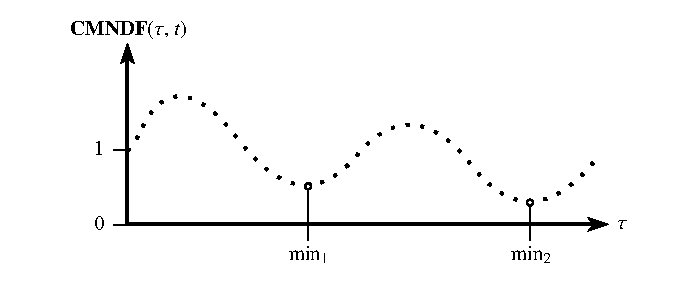
\includegraphics[width=0.8\textwidth]{papers/autotune/images/CMNDF_Minimum.pdf}
	\caption{Finden der lokalen Minima der CMNDF.}
    \label{autotune:fig:cmndfMinimum}
\end{figure}

Es fällt auf, dass die CMNDF mehrere lokale Minima aufweist.
Diese entsprechen den Vielfachen der Grundharmonischen und sind nicht von Interesse.
In der Praxis erweist es sich zum Teil als schwierig, das richtige lokale Minimum zu finden.
Oft wird deshalb ein Schwellwert definiert.
An der Stelle wo die CMNDF diesen Schwellwert unterschreitet, wird das Minimum definiert.
Dies ist im Beispiel eines realen Signals (Gesangsaufnahme) in Abbildung \ref{autotune:fig:cmndfRealSignal} ersichtlich.
\begin{figure}
	\centering
	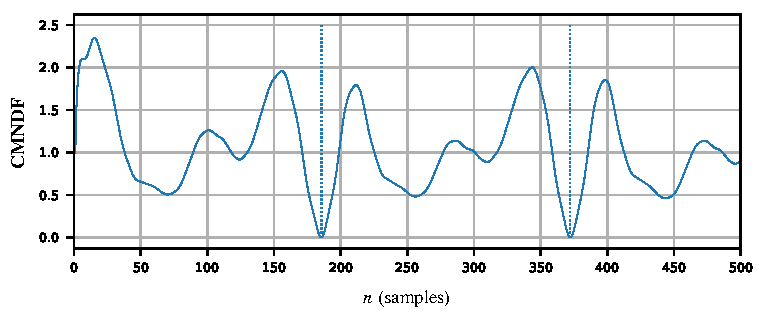
\includegraphics[width=\textwidth]{papers/autotune/images/Example-CMNDF.pdf}
	\caption{CMNDF eines realen Signals (Gesangsaufnahme) mit mehreren lokalen Minima.}
    \label{autotune:fig:cmndfRealSignal}
\end{figure}

Im Zeitbereich kann ebenfalls anschaulich dargestellt werden, wie sich das ursprüngliche Signal und die um eine Periodendauer der Grundharmonischen verzögerte Version überlagern.
Dies ist in Abbildung \ref{autotune:fig:audioShifted} ersichtlich.
\begin{figure}
	\centering
	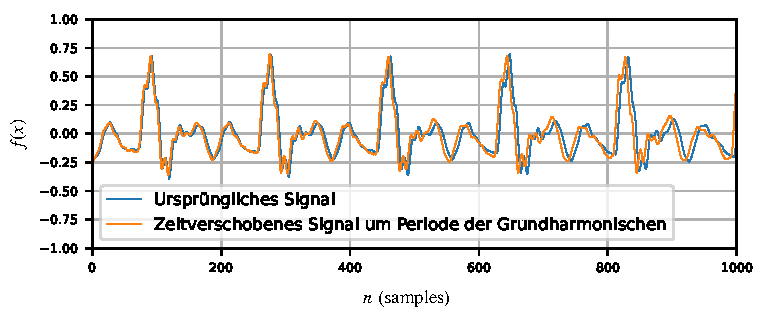
\includegraphics[width=\textwidth]{papers/autotune/images/Example-Audio-Shifted.pdf}
	\caption{Überlagerung des ursprünglichen Signals und der um eine Periodendauer der Grundharmonischen verzögerten Version.}
    \label{autotune:fig:audioShifted}
\end{figure}

Die Tonhöhe kann nun bestimmt werden als
\begin{equation}
    f_{\text{pitch}}
    =
    \frac{1}{\operatorname{min}_1}.
\end{equation}
Anders ausgedrückt wird bei der CMNDF nicht direkt die Frequenz, sondern die Periodendauer der Grundharmonischen geschätzt.
Die spektrale Frequenzauflösung ist also abhängig von der Samplefrequenz.
Bei einer typischen Samplefrequenz von 44.1\;kHz kann die Periodenlänge mit einer Genauigkeit von 22.7\;$\mu$s bestimmt werden.
Der maximale Frequenzabtastungsfehler ist somit abhängig von der Periodenlänge, also von der Tonhöhe.
Je höher die Tonhöhe, desto grösser der Frequenzabtastfehler.
Mathematisch ausgedrückt als
\begin{equation}
    f_{\text{error}}(f)
    =
    f - \frac{1}{\frac{1}{2 f_s} + \frac{1}{f}}.
\end{equation}
Der Kammerton von 440\;Hz kann bei einer Samplefrequenz von 44.1\;kHz auf ungefähr 1\;Hz genau bestimmt werden, 
was einem relativen Fehler von 0.5\% entspricht.

Die CMNDF kann im Vergleich zur STFT zudem wesentlich effizienter berechnet werden und liefert sowohl eine hohe Frequenzauflösung als auch eine hohe zeitliche Auflösung.
Dies ist in Abbildung \ref{autotune:fig:pitchDetektionCMNDF} gut ersichtlich.
\begin{figure}
	\centering
	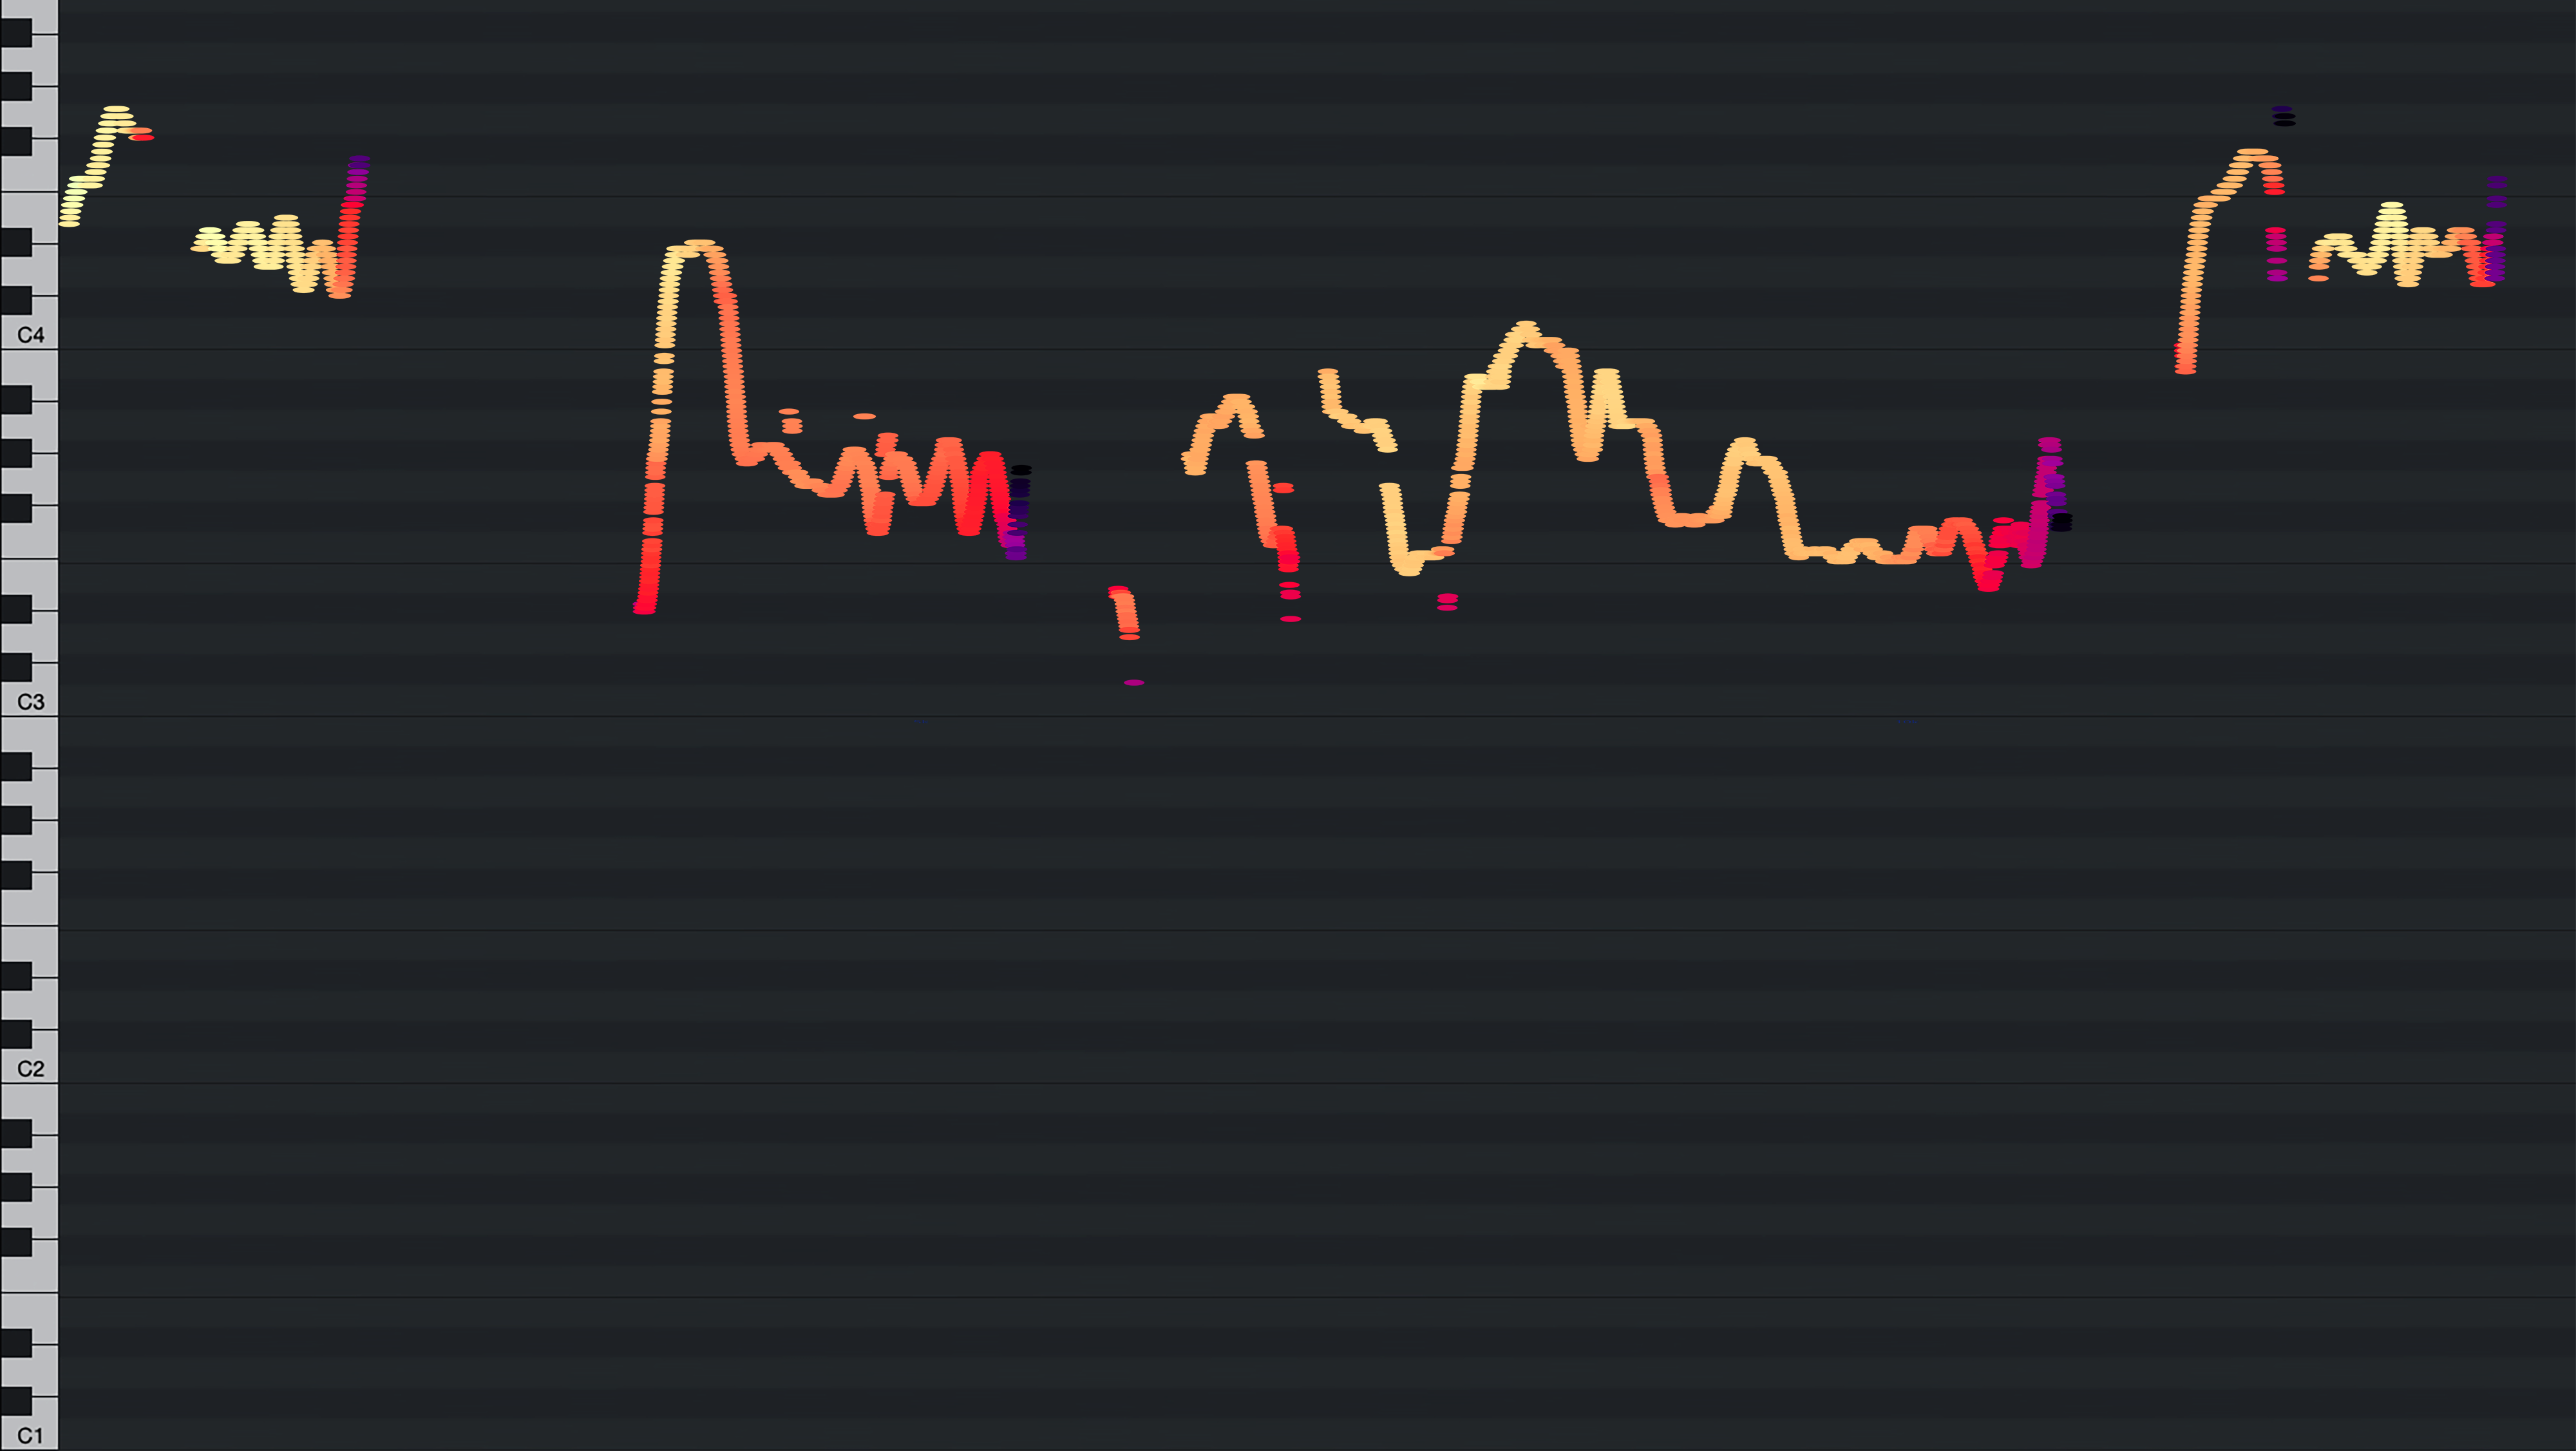
\includegraphics[width=\textwidth]{papers/autotune/images/Pianoscale_Example_Detuned_CMNDF.png}
	\caption{Pitch-Detektion mit CMNDF. Farbton entspricht dem Betrag des lokalen Minimums (je heller desto kleiner).}
    \label{autotune:fig:pitchDetektionCMNDF}
\end{figure}

Es zeigt sich, dass kommerzielle Software-Tools mit grosser Wahrscheinlichkeit die CMNDF-Methode verwenden.
So stimmen die eigens mittels CMNDF berechneten Tonhöhen mit denjenigen der kommerziellen Software \emph{Steinberg Cubase 12 Pro VariAudio} überein,
welche als Referenz verwendet wurde. Dies ist dargestellt in Abbildung \ref{autotune:fig:pitchDetektionCMNDFReference}.
\begin{figure}
	\centering
	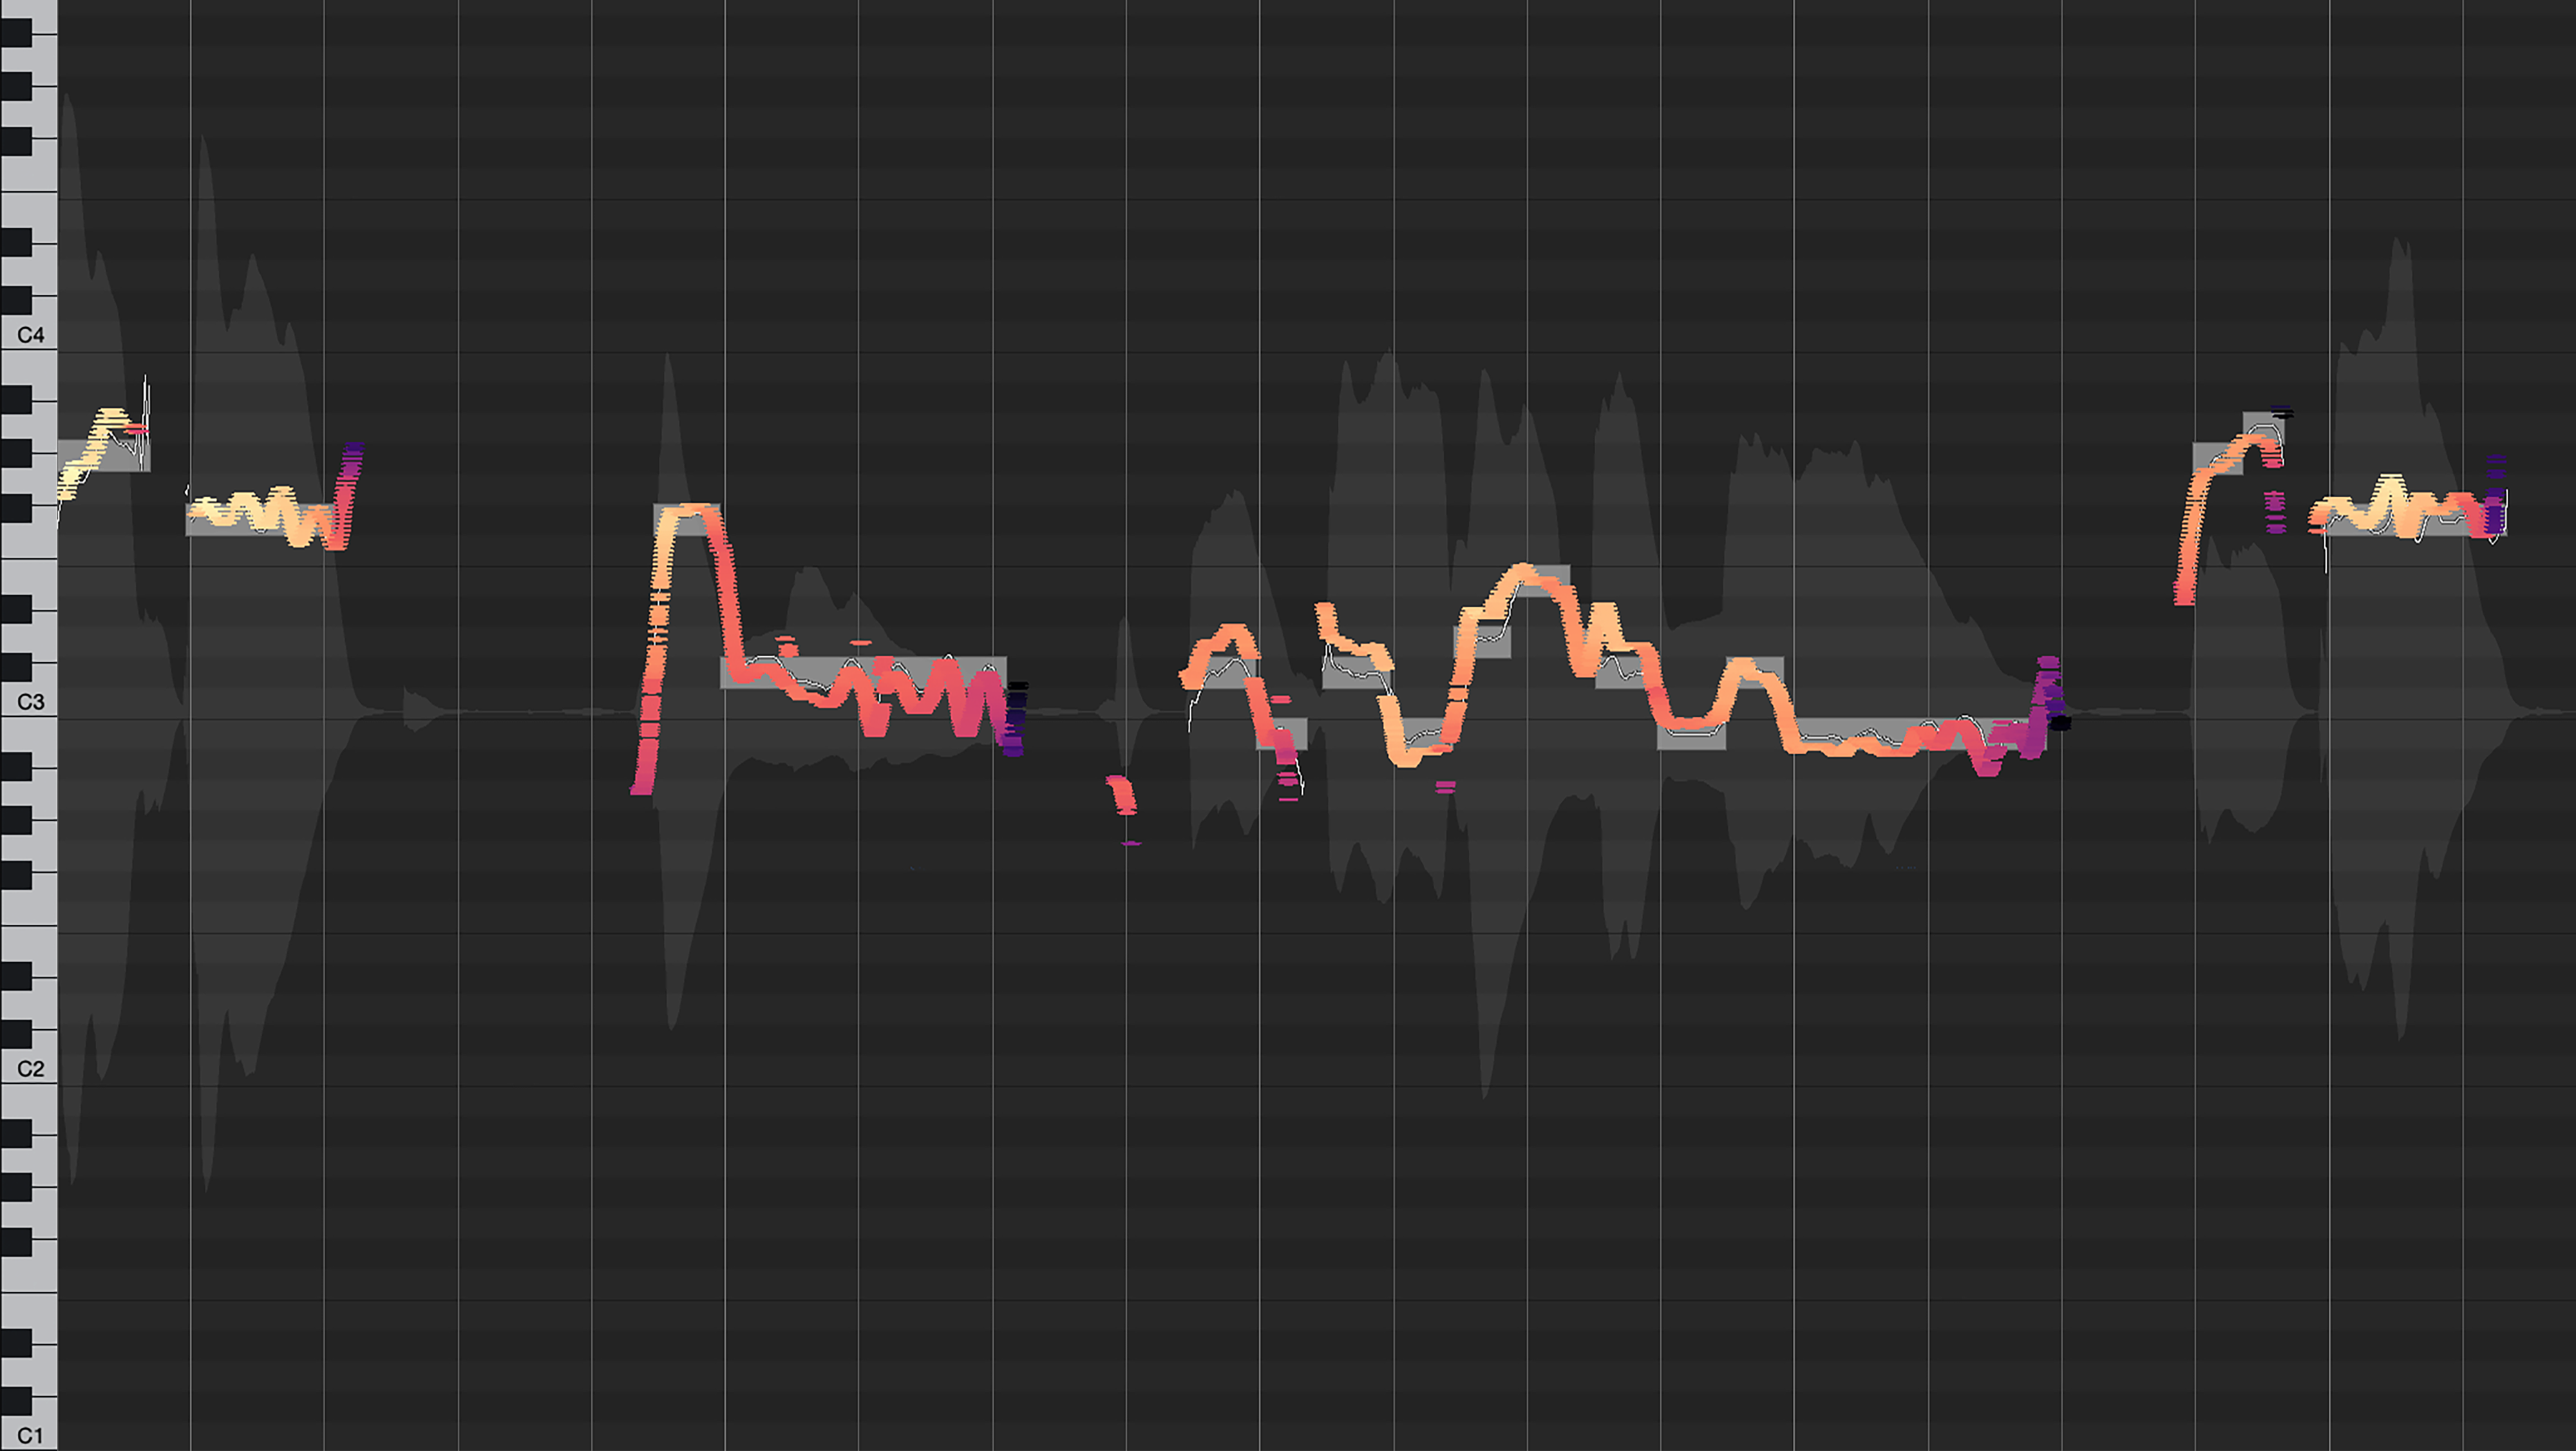
\includegraphics[width=\textwidth]{papers/autotune/images/Pianoscale_Example_Detuned_CMNDF_Reference.png}
	\caption{Vergleich der Tonhöhenbestimmung mit CMNDF und kommerzieller Auto-Tune Software (Steinberg Cubase 12 Pro VariAudio).}
    \label{autotune:fig:pitchDetektionCMNDFReference}
\end{figure}
